This article proposes two situations.
The first situation, which they call region A, proposes a very dense road network with a constant speed limit on all the road network.
The second situation, which they call region B, proposes a road network much less dense than the precedent, but with different speeds of movements.

The comparisons of these two regions base themselves on the inaccessible pairs, the length of the average route and to finish the changes of neighbors.

\begin{multicols}{2}
\textit{\textbf{Région A}}
\begin{figure}[h]
\center
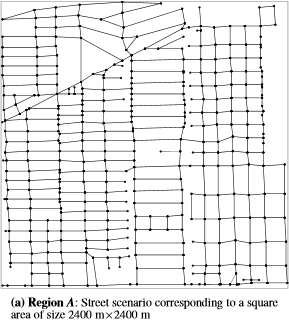
\includegraphics[width=7cm,height=50mm]{../images/cityA.png}
\caption{City application}
\end{figure}
\columnbreak
\textit{\textbf{Region B}}
\begin{figure}[h]
\center
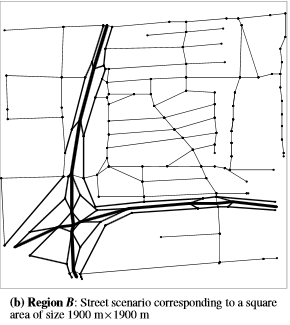
\includegraphics[width=7cm,height=50mm]{../images/cityB.png}
\caption{City application}
\end{figure}
\end{multicols}


\begin{multicols}{2}
\textit{\textbf{Région A}}
\begin{itemize}[label=$\square$]
\item Transmission range : 250 meters.
\item 200 nodes.
\item 10\% of the pairs of nodes are incapable to communicate.
\end{itemize}
\columnbreak
\textit{\textbf{Region B}}
\begin{itemize}[label=$\square$]
\item Transmission range : 250 meters.
\item 200 nodes.
\item 5\% of the pairs of knots were disconnected.
\item The connectivity is better than in the region A.
\end{itemize}
\end{multicols}